\documentclass[manuscript,screen,review]{acmart}
\AtBeginDocument{%
\providecommand\BibTeX{{%
\normalfont B\kern-0.5em{\scshape i\kern-0.25em b}\kern-0.8em\TeX}}}

\setcopyright{acmcopyright}
\copyrightyear{2018}
\acmYear{2018}
\acmDOI{XXXXXXX.XXXXXXX}

%% These commands are for a PROCEEDINGS abstract or paper.
\acmConference[Conference acronym 'XX]{Make sure to enter the correct
	conference title from your rights confirmation emai}{June 03--05,
	2018}{Woodstock, NY}
%
%  Uncomment \acmBooktitle if th title of the proceedings is different
%  from ``Proceedings of ...''!
%
\acmBooktitle{Woodstock '18: ACM Symposium on Neural Gaze Detection,
	June 03--05, 2018, Woodstock, NY}
\acmPrice{15.00}
\acmISBN{978-1-4503-XXXX-X/18/06}
%%
%% Submission ID.
%% Use this when submitting an article to a sponsored event. You'll
%% receive a unique submission ID from the organizers
%% of the event, and this ID should be used as the parameter to this command.
%%\acmSubmissionID{123-A56-BU3}

%%
%% For managing citations, it is recommended to use bibliography
%% files in BibTeX format.
%%
%% You can then either use BibTeX with the ACM-Reference-Format style,
%% or BibLaTeX with the acmnumeric or acmauthoryear sytles, that include
%% support for advanced citation of software artefact from the
%% biblatex-software package, also separately available on CTAN.
%%
%% Look at the sample-*-biblatex.tex files for templates showcasing
%% the biblatex styles.
%%

%%
%% The majority of ACM publications use numbered citations and
%% references.  The command \citestyle{authoryear} switches to the
%% "author year" style.
%%
%% If you are preparing content for an event
%% sponsored by ACM SIGGRAPH, you must use the "author year" style of
%% citations and references.
%% Uncommenting
%% the next command will enable that style.
%% \citestyle{acmauthoryear}
\usepackage{microtype}  %towards typographic perfection...
\usepackage{tikz}
\usepackage{tikz-qtree}
\usetikzlibrary{positioning}
\usetikzlibrary{arrows.meta, shapes.misc, positioning}
\usepackage{subfig}
\theoremstyle{definition}
\newtheorem{exmp}{Example}[section]
\usepackage[ruled, vlined, linesnumbered]{algorithm2e}
\SetKw{True}{true}
\SetKw{False}{false}
\SetKwData{typeInt}{Int}
\SetKwData{typeRat}{Rat}
\SetKwData{Defined}{Defined}
\SetKwFunction{parseStatement}{parseStatement}

%%
%% end of the preamble, start of the body of the document source.
\begin{document}

%%
%% The "title" command has an optional parameter,
%% allowing the author to define a "short title" to be used in page headers.
\title{A Back-to-basics Empirical Study of Datalog Materialization}

%% The "author" command and its associated commands are used to define
%% the authors and their affiliations.
%% Of note is the shared affiliation of the first two authors, and the
%% "authornote" and "authornotemark" commands
%% used to denote shared contribution to the research.
\author{Bruno Rucy Carneiro Alves de Lima}
\email{bruno.rucy.carneiro.alves.de.lima@ut.ee}
\orcid{1234-5678-9012}

\author{Kalmer Apinis}
\email{kalmer.apinis@ut.ee}
\affiliation{%
	\institution{University of Tartu}
	\city{Tartu}
	\country{Estonia}
}

%%
%% By default, the full list of authors will be used in the page
%% headers. Often, this list is too long, and will overlap
%% other information printed in the page headers. This command allows
%% the author to define a more concise list
%% of authors' names for this purpose.
\renewcommand{\shortauthors}{Trovato and Tobin, et al.}

%%
%% The abstract is a short summary of the work to be presented in the
%% article.
\begin{abstract}
	The core reasoning task for datalog engines is materialization, the
	act of evaluating a program until no more data can be inferred from
	a database. Due to it being a costly operation, it is a must for datalog
	engines to provide incremental materialization, that is, to adjust the
	computation to new data, instead of restarting from scratch. Deleting data
	is notoriously more involved than adding, since one has to take into account
	all possible data that has been inferred from what is being deleted, hence, it is
	likely that performance is not even across the direction of the update. In this
	article we investigate the performance of materialization in both directions, with
	three reference datalog implementations, out of which one is built on top of a
	lightweight relational engine, and another that uses a promising distribution framework
	for incremental computation with first-class support for recursion, that efficiently
	handles addition and deletion of data in the same way. To ensure a fair evaluation, the
	output of the paper is coalesced as an extensible reasoning framework, that shares
	as much code as it is sensible between the implementations, therefore providing strong
	evidence to the efficiency of each measure.
\end{abstract}


\keywords{datalog, incremental view maintenance, differential dataflow}

\maketitle

\section{Introduction}
\textbf{Motivation.} SQL\cite{key} has been the \textit{de facto} universal relational
database interface for querying and management since its inception,
with all other alternatives having had experienced disproportionately
little interest. The reasons for this are many, out of which only one
is relevant to this narrative; performance.

The runner-ups of popularity were languages used for machine reasoning,
a subset of the Artificial Intelligence field that attempts to attain
intelligence through the usage of rules over knowledge. The canonical
language for reasoning over relational databases is datalog\cite{datalog}.
Similarly to SQL, it also is declarative, however, its main semantics' difference
is in the support for recursion while still ensuring termination irrespective
of the program being run.

A notable issue with respect to real-world adoption of datalog is in
performance. The combined complexity of evaluating a program is
$\text{EXPTIME}$\cite{datalog}, while SQL queries are $\text{AC}^0$. It was
not until recently\cite{rdfox} that scalable implementations were
developed.

Digital analytics has been one of the main drivers of the recent datalog renaissance,
with virtually all big-data oriented datalog implementations having had either been built
on top of the most mainstream industry oriented frameworks\cite{bigdatalog,cog,cog2} or with the
aid of the most high-profile technology companies\cite{logica,yedalog,vadalog}.

Another strong source of research interest has been from the knowledge graph community. A
knowledge graph \textit{KG} is a regular relational database \textit{I} that contains
\textit{ground truths}, and rules.

The most important datalog operation is called \textit{materialization}, the derivation of all
truths that follow from the application of rules over the relational database, with the most
straightforward goal being to ensure queries do not need any reasoning.

\textbf{Problem.} The maintenance of materialization is possibly the most important issue
that plagues the real-world usage of datalog, and has been a source of much research interest,
most commonly under the guise of incremental view maintenance.

The handling of additions is efficiently done with the semi-naive evaluation method\cite{sne},
that can be notoriously efficient for a special class of programs that are popular in practice.
Deletions on the other hand, are possibly much less efficient, since the retraction of a \textit{ground truth}
naively implies the deletion of all data derived from it.

The quintessential algorithm for computing the materialization adjustment with respect to a
deletion is the delete-rederive\cite{dred} method, that generates new datalog programs to
compute the deletions necessary to ensure correctness, doing so by first computing all possible
deletions, and then all possible alternative derivations, with the adjusment being the difference
between both of these sets.

The fact that two different algorithms are used implies that there are two different performance
characteristics for additions and deletions, in spite of dred utilizing semi-naive evaluation as well,
therefore there being possibly-severe biases in performance. To this date, there hasn't been
a study that evaluated a datalog engine performance in properly dynamic scenarios.

A promising computation framework that could be well-suited to this problem is differential
dataflow\cite{differential_dataflow}. Timely dataflow is a high-throughput, low-latency
streaming-and-distributed computational model that extends the dataflow paradigm. The timely
in its name refers to it thoroughly establishing the semantics of each aspect of communication
notification, taking the parallelization blueprint and making its execution transparent to the user.

A notification sent between operators is assigned a timestamp, that needs only to be partially
ordered, with no assumptions being made with respect to insertion. The goal is to use these to
correctly reason about the data with respect to the local operator states' of computation completion,
in order to cleverly know with certainty when not only whether should work be done asynchronously
or with sharding, but whether there is data yet to be processed or not.

Differential Dataflow, a generalization of incremental processing, is an extension to the
Timely Dataflow model. While the shape of the data that flows in the latter is in the form
of \verb|(data, timestamp)|, the former's is \verb|(data, timestamp, multiplicity)|, therefore
restricting its bag-of-data semantics to multisets, with the multiplicity element representing a
difference, for instance, $+1$ representing the addition of $1$ datapoint arriving at a
specific timestamp, or $-1$, a deletion.

The key difference between both models is that similarly to how timely makes distribution
transparent, differential does the same with incremental computation, by providing to the user the
possibility of not only adding to a stream, the only possible action in timely dataflow, but
allow it to respond to arbitrary additions and retractions at any timestamp.  There is one
reasoner that uses differential dataflow\cite{ddlog}, however, it has no storage layer, instead
it compiles fixed datalog programs into fixed differential dataflow programs, that can only run in one computer.

The lack of a canonical open-source implementation of datalog makes attempts at making
empirical statements about performance-impacting theoretical developments, such as the usage of
differential dataflow, brittle and difficult, since there is no point of reference to
compare and validate, and comparisons against commercial implementations are not
reliable, since optimizations might be trade secrets.

A notorious exploration that highlights this issue is the COST, Configuration That Outperforms
a Single Thread, article\cite{COST}, in which the author posits that multiple published
graph-processing engines are likely never able to outperform simple single-threaded implementations.
Some high-profile datalog implementations were built upon systems mentioned on that article.
Later on, the author made multiple pieces of informal writing in which the most performant datalog
engines were investigated for COST\cite{blogdynamicdatalog, blogvldbsigmod}, with results that
showed a very different picture than the ones depicted by the original articles.

\textbf{Methodology.} To address the aforementioned problem, we conduct a back-to-basics
empirical study of datalog program materialization, revisiting and measuring the core assumptions
that go into the implementation of a reasoner. We coalesce this knowledge into a framework
that provides multiple shared components for reasoning research. Straightforward single-threaded,
parallel and distributed implementations, with the last being done with differential dataflow, of
both substitution-based and relational-algebra interpretations are realized alongside common
well-known optimizations.

\textbf{Contributions.} In this article we make several contributions to clarifying, benchmarking
and easing pushing the boundaries of datalog evaluation engineering research further by
providing performant and open-source implementations of single-threaded, parallel and distributed evaluators.

\begin{itemize}
	\item \textbf{Techniques and Guidelines.} We study the challenge of building a reasoner from scratch,
	      with no underlying framework, and ponder over all decisions necessary in order to bring that to fruition,
	      alongside with relevant recent literature.
	\item \textbf{Differential Dataflow.} We accurately investigate the suitability of differential
	      dataflow for datalog, and showcase how does it fare against the ubiquitous DRED and semi-naive
	      evaluation based reasoners with the same language, base and with the same data format.
	\item \textbf{Framework.} All code outputs of this article are coalesced in a rust library named shapiro,
	      consisted of a datalog to relational algebra rewriter, a relational algebra evaluator, and two datalog engines,
	      one that is parallel-capable and supports both substitution-based and relational algebra methods, and other that
	      relies on the state-of-the-art differential dataflow\cite{differential_dataflow} distribution computation framework.
	      The main expected outcome of this library is to provide well understood and reasoned about baseline implementations
	      from where future research can take advantage of, and reliable COST configurations can be attained.
	\item \textbf{Benchmarking.} We perform two thorough benchmark suites. One evaluates the performance of the developed
	      relational reasoner with multiple different index data structures and common optimizations, such as string interning
	      and simple parallelism, and another that attempts to attain the COST of the reasoner built on top of differential
	      dataflow. The selected datasets are either from the program analysis, heavy users of not-distributed datalog, or from
	      the semantic web community, which has multiple popular infinitely-scalable benchmarks.
\end{itemize}

\section{Related Work}

\textbf{Datalog engines.} There are two kinds of recent relevant datalog engines. The first encompasses
those that push the performance boundary, with the biggest proponents being RDFox\cite{rdfox}, that
proposes the to-date, according to their benchmarks, most scalable parallelisation routine, RecStep\cite{recstep},
that builds on top of a highly efficient relational engine, and DCDatalog\cite{dcdatalog}, that builds upon
an influential query optimizer, DeALS\cite{deals} and extends a work that establishes how some linear
datalog programs could be evaluated in a lock-free manner, to general positive programs.

One of the most high-profile datalog papers of interest has been BigDatalog\cite{bigdatalog}, that
originally used the query optimizer DeALs, and was built on top of the very popular Spark\cite{spark}
distribution framework. Soon after, a prototypical implementation\cite{cog} over Flink\cite{flink},
a distribution framework that supports streaming, Cog, followed. Flink, unlike Spark, supports
iteration, so implementing reasoning did not need to extend the core of the underlying framework. The most
successful attempt at creating a distributed implemention has been Nexus\cite{nexus}, that is also built on Flink,
and makes use of its most advanced feature, incremental stream processing. To date, it is the fastest distributed
implementation.

\textbf{Data structures used in datalog engines.} The core of each datalog engine is consisted of possibly
two main data structures: one to hold the data itself, and another for indexes. Surprisingly little regard is given to
this, compared to algorithms themselves, despite potentially being one of the most detrimental factors for performance
. Binary-decision diagrams\cite{bddbddb}, hash sets\cite{microzee} and B-Trees\cite{souffle_btree} are often used as
either one or both main structures. An important highlight of the importance of data structure implementation is how
in \cite{souffle_btree} Subotic et al, managed to attain an almost 50 times higher performance in certain benchmarks
than other implementations of the same data structure.

\section{Datalog Evaluation}

In this section we review the basics of all concepts related to datalog evaluation, as it is done in the current time.

\subsection{Datalog}

\textit{Datalog}\cite{all_you_ever_wanted_to_ask} is a declarative programming language. A program $P$ is a set of
rules $r$, with each $r$ being a restriction of tuple-generating dependencies: \[\bigwedge_{i=1}^kB_i(x_1, ..., x_j) \rightarrow \exists (y_1, ..., y_j)H(x_1, ..., x_j, y_1, ..., y_j)\]
with $k$, $j$ as finite integers, $x$ and $y$ as terms, and each $B_i$ and $H$ as predicates. A term can belong
either to the set of variables, or constants, however, it is to be noted that all $y$ are existentially quantified.
The set of all $B_i$ is called the \textit{body}, and $H$ the \textit{head}.

A rule $r$ is said to be datalog, if the set of all $y$ is empty, and no predicate is negated, conversely, a
datalog program is one in which all rules are datalog.
\begin{exmp}{Datalog Program}\label{ex1}
	\[
		P = \left\{  \begin{array}{l}
			\text{SubClassOf}(?x, ?y) \wedge \text{SubClassOf}(?y, ?z) \rightarrow \text{SubClassOf}(?x, ?z) \\
		\end{array}\right\}
	\]
\end{exmp}
Example \ref{ex1} shows a simple valid recursive program. The only rule denotes that \textit{for all x, y, z, if x is
	in a SubClassOf relation with y, and y is in a SubClassOf relation with z, then it follows that x is in a subClassOf
	relation with z}.

The meaning of a datalog program is often\cite{datalog} defined through a \textit{Herbrand Interpretation}. The first step
to attain it is the \textit{Herbrand Universe} $\mathfrak{U}$, the set of all constant, commonly referred to as \textit{ground}, terms.
\begin{exmp}{Herbrand Universe}\label{ex2}
	\[
		S = \left\{ \begin{array}{l}
			\text{SubClassOf}(\text{professor}, \text{employee}) \\
			\text{SubClassOf}(\text{employee}, \text{taxPayer})  \\
			\text{SubClassOf}(\text{employee}, \text{employed})  \\
			\text{SubClassOf}(\text{employed}, \text{employee})
		\end{array}\right\}
	\]
	\[
		\mathfrak{U} = \left\{  \begin{array}{l}
			\text{professor}, \text{employee}, \text{employed}, \text{taxPayer}
		\end{array}\right\}
	\]
\end{exmp}
From the shown universe on example \ref{ex2}, it is possible to build The \textit{Herbrand Base}, the set of all possible truths,
from \textit{facts}, assertions that are true, as represented by the actual constituents of the SubClassOf set.
\begin{exmp}{Herbrand Base}\label{ex3}
	\[
		\mathfrak{B} = S \cup \left\{  \begin{array}{l}
			\text{SubClassOf}(\text{professor}, {professor}) \\
			\text{SubClassOf}(\text{employee}, {employee})   \\
			\text{SubClassOf}(\text{employed}, {employed})   \\
			\text{SubClassOf}(\text{taxPayer}, {taxPayer})   \\
			\text{SubClassOf}(\text{professor}, {taxPayer})  \\
			\text{SubClassOf}(\text{taxPayer}, {professor})  \\
			\text{SubClassOf}(\text{employee}, {professor})  \\
			\text{SubClassOf}(\text{taxPayer}, {employee})
		\end{array}\right\}
	\]
\end{exmp}
On example \ref{ex3}, all facts are indeed \textit{possible}, but not necessarily \textit{derivable} from the actual data and
program. An interpretation $I$ is a subset of $\mathfrak{B}$, and a \textit{model} is an interpretation such that all rules
are satisfied. A rule is satisfied if either the head is true, or if the body is not true.
\begin{exmp}{Models}\label{ex4}
	\[
		I_1 = S \cup \left\{  \begin{array}{l}
			\text{SubClassOf}(\text{professor}, {taxPayer}) \\
			\text{SubClassOf}(\text{employee}, {employee})
		\end{array}\right\}
	\]
	\[
		I_2 = S \cup \left\{  \begin{array}{l}
			\text{SubClassOf}(\text{professor}, {taxPayer}) \\
			\text{SubClassOf}(\text{employee}, {employee})  \\
			\text{SubClassOf}(\text{employed}, {employed})
		\end{array}\right\}
	\]
	\[
		I_3 = S \cup \left\{  \begin{array}{l}
			\text{SubClassOf}(\text{professor}, {taxPayer}) \\
			\text{SubClassOf}(\text{employee}, {employee} ) \\
			\text{SubClassOf}(\text{employed}, {employed})  \\
			\text{SubClassOf}(\text{professor, professor})
		\end{array}\right\}
	\]
\end{exmp}
The first interpretation, $I_1$, from example \ref{ex4}, is not a model, since $\text{SubClassOf}(\text{employed}, \text{employed})$ is satisfied
and present. Despite both $I_2$ and $I_3$ being models, $I_2$ is the \textit{minimal} model, which is the definition of the meaning of the program
over the data. The input data, the database, is named as the \textit{Extensional Database} $EDB$, and the output of the program is the \textit{Intensional Database}
$IDB$.

Let an $DB = EDB \cup IDB$, and for there to be a program $P$. We define the \textit{immediate consequence} of $P$ over $DB$ as all facts
that are either in $DB$, or stem from the result of applying the rules in $P$ to $DB$. The \textit{immediate consequence operator}
$\textbf{I}_C(DB)$ is the union of $DB$ and its immediate consequence, and the $IDB$, at the moment of the application of $\textbf{I}_C(DB)$
is the difference of the union of all previous $DB$ with the $EDB$.


It is trivial to see that $I_C(DB)$ is monotone, and given that both the $EDB$ and $P$ are finite sets, and that $IDB = \emptyset$ at the start,
at some point $I_C(DB) = DB$, since there won't be new facts to be inferred. This point is the \textit{least fixed point} of $I_c(DB)$\cite{datalog},
and happens to be the \textit{minimal} model.
\begin{exmp}{Repeated application of $I_c$}
	\begin{align}
		P = \{ Edge(?x, ?y) \leftarrow TC(?x, ?y), TC(?x, ?y), TC(?y, ?z) \leftarrow TC(?x, ?z) \} \nonumber             \\
		EDB = \{ Edge(1, 2), Edge(2, 3), Edge(3, 4) \}                                               \nonumber           \\
		DB = EDB                                                                                     \nonumber           \\
		DB = I_C(DB)                                                                                                     \\
		DB == EDB \cup \{ TC(1, 2), TC(2, 3), TC(3, 4) \}                                                      \nonumber \\
		DB = I_C(DB)                                                                                           \nonumber \\
		DB == EDB \cup \{ TC(1, 2), TC(2, 3), TC(3, 4), TC(1, 3), TC(2, 4) \}                                  \nonumber \\
		DB = I_C(DB)                                                                                                     \\
		DB == EDB \cup \{ TC(1, 2), TC(2, 3), TC(3, 4), TC(1, 3), TC(2, 4), TC(1, 4) \}                        \nonumber \\
		DB = I_C(DB)                                                                                                     \\
		DB == EDB \cup \{ TC(1, 2), TC(2, 3), TC(3, 4), TC(1, 3), TC(2, 4), TC(1, 4) \}                        \nonumber \\
		IDB = DB \setminus EDB
	\end{align}
	\label{ex5}
\end{exmp}

The walkthrough given on example \ref{ex5} is called \textit{naive} evaluation. Every number indicates one rendering of the immediate consequence. As it can be seen by 3 and 4, at some point $DB$ equals $I_C(DB)$, from which onwards no more new tuples will be inferred, therefore halting.

The ubiquitous evaluation mechanism, as of the date of writing this paper, is the \textit{semi-naive} one. The difference is that \textit{semi-naive} does not repeatedly union the $EDB$ with the entire $IDB$, but does so only with the difference of the previous immediate consequence with the $IDB$. This can be hinted from the example, where each next application of $I_c$ only renders new facts from the previous newly derived ones.

\subsection{Infer}
The most relevant performance-oriented aspect of both of the introduced evaluation mechanisms is the implementation of $I_c$ itself. The two
most high-profile methods to do so are either purely evaluating the rules, or rewriting them in some other imperative formalism, and executing it.

The Infer\cite{datalog} method is the simplest example of the former, and relies on substitutions. A substitution $S$ is a homomorphism
$[x_1 \rightarrow y_1, ..., x_i \rightarrow y_i]$, such that $x_i$ is a variable, and $y_i$ is a constant. Given a not-ground fact,
such as $TC(?x, 4)$, \textit{applying} the substitution $[?x \rightarrow 1]$ to it will yield the ground fact $TC(1, 4)$.

Infer relies on attempting to build and extend substitutions for each fact in each rule body over every single $DB$ fact. Once
all substitutions are made, they are applied to the heads of each rule. Every result of this application that is ground belongs
to the immediate consequence.

\subsection{Relational Algebra}
Relational Algebra\cite{codd_1970} explicitly denotes operations over sets of tuples with fixed arity, relations. It is
the most popular database formalism that there is, with virtually every single major database system adhering to the relational model\cite{pg,mysql,sqlserver}
and using SQL as a declarative syntax for relational algebra.

Let $R$ and $T$ be relations with arity $r$ and $t$, $\theta$ be a binary operation with a boolean output, $R(i)$ be the i-th column, all terms in the i-th position of every tuple in $R$, and
$R[h, ..., k]$ be the subset of $R$ such that only the columns $h, ..., k$ remain, and Const the set of all constant terms. The following
are the most relevant relational algebra operators and their semantics:
\begin{itemize}
	\item Selection by column $\sigma_{i=j)}(R) = \{ a \in R | a(i) == a(j) \}$
	\item Selection by value $\sigma_{i=k}(R) = \{a \in R | a(i) == k \}$
	\item Projection $\pi_{h, ..., k}(R) = \{(R(i), ..., R(j), \overrightarrow{C}) |  i, j >= 1 \wedge i, j <= r\ \wedge \forall c \in C. c \in \text{Const}$
	\item Product $\times(R, T) = \{(a, b) | a \in R \wedge b \in T \}$
	\item Join $\Join_{i=j} = \{(a, b) | a \in R \wedge b \in T \wedge a(i) == b(j)\}$
\end{itemize}

Rewriting datalog into some form of relational algebra has been the most successful strategy employed by the vast majority of all current state-of-the-art
reasoners\cite{bigdatalog, cog, nexus, recstep, dcdatalog, souffle} mostly due to the extensive industrial and academic research into developing data processing frameworks that
process very large amounts of data, and the techniques that have arisen from these.

In spite of this, there is no open-source library that provides a stand-alone datalog to relational algebra translator, therefore every single
datalog evaluator has to repeat this effort. Moreover, datalog rules translate to a specific form of relational algebra expressions, the
select-project-join $\mathcal{SPJ}$ form.

A relational algebra expression is in the $\mathcal{SPJ}$ form if it consists solely of select, project and join operators. This form
is very often seen in practice, being equivalent to \verb|SELECT ... FROM ... WHERE ...| SQL queries, and highly benefits from being
equivalent to conjunctive queries, that are equivalent to single-rule and non-recursive datalog programs.

We propose a straightforward not-recursive pseudocode algorithm to translate a datalog rule into a $SPJ$ expression tree, in which
relational operators are nodes and leaves are relations. The value proposition of the algorithm is for the resulting tree to be ready
to be recursively executed, alongside having two essential relational optimizations, selection by value pushdown, and melding selection
by column with products into joins, the most important relational operator. This is paramount to understanding the performance of the relational reasoner.

The algorithm has two parts, generating a semantically equivalent relational expression to the input rule, and then optimising all products out for joins, therefore turning it into a $\mathcal{SPJ}$ expression.

\begin{algorithm}
	\scriptsize
	\KwIn{A datalog rule $\mathcal{R}$}
	\KwResult{A relational algebra expression $\mathcal{R}_a$}
	\SetKwData{s}{s}
	\BlankLine
	\SetKwProg{Fn}{Function}{ is}{end}
	\SetKwProg{For}{For}{:}{end}

	\Fn{toIncompleteExpression($r$ : Datalog Rule)}{
		let $t$ be a fresh tree

		\For{every fact $a_i$ in the rule body $b$} {
			create a relation node $r_i$ with the same arity as $a_i$, and its terms representing columns. variable terms
			are column identifiers, and constant terms are temporary-lived proxies for selections.
			\If {$i < len(b) - 1$ } {
				add a product node $p_i$ to $t$.
				set $r_i$ as the left child of $p_i$.
			}\Else {
				\If {$len(b) > 1$} {
					set $r_i$ as the right child of $p_{i - 1}$
				}
			}
			\If {$i > 0$} {
				set $p_i$ as the right child of $p_{i - 1}$
			}
		}
		\textbf{return} $t$
	}
	\caption{toIncompleteExpression procedure}
	\label{alg:to_incomplete_expression}
\end{algorithm}

Procedure \ref{alg:to_incomplete_expression} receives as input a rule, such as $TC(?x, z) \leftarrow TC(?x, y), TC(y, ?z)$, and outputs an
incomplete expression tree representing a relational inclusion comprised solely of products: $(TC(?x, y) \times TC(y, ?z)) \subseteq TC$.

\begin{algorithm}
	\scriptsize
	\KwIn{A datalog rule $\mathcal{R}$}
	\KwResult{A relational algebra expression $\mathcal{R}_a$}
	\SetKwData{s}{s}
	\BlankLine
	\SetKwProg{Fn}{Function}{ is}{end}
	\SetKwProg{For}{For}{:}{end}

	\Fn{constantToSelection($e$ : Expression)}{
		let $t$ be a copy of $e$

		let $C$ be a map $C : \text{Const} \rightarrow \text{Var}$

		\For {every relation $r_i$ in $t$} {
			\For {every constant $c_j$ in $r_i$}{
				add a selection by value node $s_j$ to $t$ with column index $j$ and value $c_j$

				set $s_j$'s parent to $r_i$'s, and $r_i$ as its left child

				\If {$\neg (c_j \in C)$}{
					create a fresh variable term $v_j$ and store it in $C$ with $c_j$ as the key}
				\Else{replace $c_j$ for the value in $C$ under $c_j$}
			}
		}
		\textbf{return} $t$
	}
	\caption{constantToSelection procedure}
	\label{alg:constant_to_selection}
\end{algorithm}

The next two steps handle the translation of datalog constant terms into selection operations. procedure \ref{alg:constant_to_selection} will swap out
all constant terms in relations for selections by value, that will remain as close as possible to the relation node: $(\sigma_{1=y}TC(?x, ?y) \times \sigma_{0=y}TC(?y, ?z)) \subseteq TC$.

\begin{algorithm}
	\scriptsize
	\KwIn{A datalog rule $\mathcal{R}$}
	\KwResult{A relational algebra expression $\mathcal{R}_a$}
	\SetKwData{s}{s}
	\BlankLine
	\SetKwProg{Fn}{Function}{ is}{end}
	\SetKwProg{For}{For}{:}{end}

	\Fn{equalityToSelection($e$ : Expression)}{
		let $t$ be a copy of $e$

		let $V$ be a map $V : \text{Var} \rightarrow \mathbb{Z}$

		let $t_{p}$ be a pre-order traversal of $t$

		\For {every relation $r_i$ in $t_{p}$} {
			\For {every variable $v_j$ in $r_i$}{
				\If{$\neg (v_j \in V)$}{
					add $v_j$ to $V$ with $j$ as the value
				}\Else{let $k$ be the value of $v_j$ in $V$
					let $p_i$ be the first product to the left of $r_i$ in $t_{p}$

					add a selection by column node $s_j$ to $t$ with left column index $k$ and right column index $j$

					set $s_j$'s parent to $p_i$'s, and $p_i$ as its left child
				}
			}
		}
		\textbf{return} $t$
	}
	\caption{equalityToSelection procedure}
	\label{alg:equality_to_selection}
\end{algorithm}

With constant terms being gone, it is necessary to remove variable terms altogether. This is done with procedure \ref{alg:equality_to_selection}, that
whenever there are terms with the same symbol, a selection by column is added: $(\sigma_{1=2}(\sigma_{1=y}TC \times \sigma_{0=y}TC)) \subseteq TC$.

\begin{algorithm}
	\scriptsize
	\KwIn{A datalog rule $\mathcal{R}$}
	\KwResult{A relational algebra expression $\mathcal{R}_a$}
	\SetKwData{s}{s}
	\BlankLine
	\SetKwProg{Fn}{Function}{ is}{end}
	\SetKwProg{For}{For}{:}{end}

	\Fn{projectHead($e$ : Expression, $r$ : Datalog Rule)}{
		let $n$ be 0

		let $t$ be a copy of $e$

		let $h$ be the head of $r$

		let $t_{p}$ be a pre-order traversal of $t$

		let $V$ be a map $V : \text{Var} \rightarrow \mathbb{Z}$

		\For {every relation $r_i$ in $t_{p}$}{
			\For {every term $x$ in $r_i$}{
				\If {$x$ is a variable} {
					add $x$ to $V$ with $n$ as value
				}\Else{
					continue
				}
				$n$ += 1

				add projection node $z$ to $t$ and set it as root with an empty list

				\For {every term $x$ in $h$}{
					\If {$x$ is a constant}{
						push $x$ into $z$
					}\Else {
						let $k$ be the value of $x$ in $V$

						push $k$ into $z$
					}
				}
			}
		}

		\textbf{return} $t$
	}
	\caption{projectHead procedure}
	\label{alg:project_head}
\end{algorithm}

The last step in translation is the most straightforward one, to convert the head of the rule. This is directly done with procedure \ref{alg:project_head} by converting the head $TC(?x, ?z)$ into a relational projection node: $\pi_{[0, 2]}(\sigma_{1=2}(\sigma_{1=y}TC \times \sigma_{0=y}TC)) \subseteq TC$. Now, the output expression is semantically equivalent to the input rule.

\begin{algorithm}
	\scriptsize
	\KwIn{A datalog rule $\mathcal{R}$}
	\KwResult{A relational algebra expression $\mathcal{R}_a$}
	\SetKwData{s}{s}
	\BlankLine
	\SetKwProg{Fn}{Function}{ is}{end}
	\SetKwProg{For}{For}{:}{end}
	\Fn{productToJoin($e$ : Expression)}{
		let $t$ be a copy of $e$

		let $t_{p}$ be a pre-order traversal of $t$

		\For {every selection by column $s_i$ in $t_{p}$}{
			find the first product $p_j$ after $s_i$ in $t_{p}$

			remove $s_i$ from $t$, swap $p_j$ for a join $g_j$ in $t$ with left and right column indexes by those of $s_i$
		}
		\textbf{return} t
	}

	\textbf{return} $\mathcal{R}_a$
	\caption{productToJoin procedure}
	\label{alg:product_to_join}
\end{algorithm}

The second part of the algorithm is brief, yet of paramount importance, as it optimises all products away into joins with procedure \ref{alg:product_to_join}: $\pi_{[0, 2]}(\sigma_{1=y}TC \Join_{1=2} \sigma_{0=y}TC) \subseteq TC$.

The canonical algorithms for translating datalog to relational algebra\cite{opt_sys_alg_ev_dat, log_dab} are recursive, complex,
and do not assume the output to be a tree, instead being mostly symbolic.

\section{DRED}

The regular semi-naive evaluation method is already incremental, and easily handles the addition of data. One merely has to continue the evaluation with all previous data as the most recent delta.

The most used method for handling deletions is a bottom-up algorithm\cite{dred} that uses semi-naive evaluation to evaluate two new programs, one that computes all possible deletions that could stem from the deletion of the facts being retracted, and then another that attempts to find alternative derivations to the overdeleted ones.

Given a program $P$ with rules $r_0, ..., r_n$, with bodies $b(r) = \{b_0, ..., b_k\}$ and heads $h(r)$, the overdeletion program will generate one new $-$rule for each $b_j$ in each rule body $b(r_i)$, in order to represent that if such fact were to be deleted, then $h(r_i)$ would not hold true.

\begin{exmp}{DRED Overdeletion program}
	\begin{align}
		P = \{ TC(?x, ?z) \leftarrow Edge(?x, ?y), TC(?y, ?z); TC(?x, ?y) \leftarrow Edge(?x, ?y) \} \nonumber                                                \\
		-r_0 = -TC(?x, ?y) \leftarrow -Edge(?x, ?y)                                                                                                           \\
		-r_1 = -TC(?x, ?z) \leftarrow -Edge(?x, ?y), TC(?y, ?z)                                                                                     \nonumber \\
		-r_2 = -TC(?x, ?z) \leftarrow Edge(?x, ?y), -TC(?y, ?z)
	\end{align}
	\label{ex6}
\end{exmp}

On example \ref{ex6} negative predicates represent overdeletion targets. For instance, if \verb|Edge(2, 3)| is being deleted, then \verb|TC(2, 3)| will be deleted, and any other inferred fact that depends on it. Given that it is a regular datalog program, it can be efficiently evaluated with semi-naive evaluation.

The next step is to compute the alternative derivations of the deleted facts, since some overdeleted facts might still hold true. The alternative derivation program will generate one new $+$rule for each $r_i$ in $P$, with one extra $-$ head predicate per body, representing an overdeleted fact. The $+$ program requires the overdeleted facts to not be present.

\begin{exmp}{DRED Overdeletion program}
	\begin{align}
		P = \{ TC(?x, ?z) \leftarrow Edge(?x, ?y), TC(?y, ?z); TC(?x, ?y) \leftarrow Edge(?x, ?y) \} \nonumber                                                           \\
		r_0 = +TC(?x, ?y) \leftarrow -TC(?x, ?y), Edge(?x, ?y)                                                                                                           \\
		r_1 = +TC(?x, ?z) \leftarrow -TC(?x, ?z), Edge(?x, ?y), TC(?y, ?z)                                                                                     \nonumber \\
	\end{align}
	\label{ex7}
\end{exmp}

The output relations from example \ref{ex7} represent the data that has to be put back into the materialization. The rationale for alternative derivations is that, for $r_1$, for instance, if the edge \verb|TC(3, 4)| was overdeleted, because of there being \verb|Edge(1, 2)| and \verb|TC(2, 3)|, if \verb|Edge(3, 4)| was not deleted, by rule $r_0$, then there is an alternative derivation for \verb|TC(3, 4)|.

As it can be seen, computing the maintenance of the materialization implies evaluating a program bigger than the materialization itself, however, due to the fact that it is evaluated with semi-naive evaluation in itself, the asymptotic complexity remains the same\cite{complexity_of_dred}. Nonetheless, in practice, deletion is often much slower than addition.

\section{Shapiro}
The central contribution of this article is Shapiro, an extensible reasoning system designedfrom scratch. No frameworks
were used, nor any code related to any other reasoner has been reutilized, furthermore, a modern, performant and safe programming
language was used, Rust\cite{rust_lang}.

All most performant shared-memory reasoners are unsurpisingly all implemented in C++\cite{rdfox, vadalog, souffle}, since
it provides manual memory management and is the \textit{de facto} language for high-performance computing. Rust is a
recent language, approximately 10 years old, that exhibits similar or faster performance than C++, with its \textit{raison d'etre}
being that, unlike C++, it is memory-safe and thread-safe\cite{rust2014,rustbelt,rustsafety}; both of these guarantees are
of incredible immediate benefit to writing a reasoner.

Shapiro, the developed system, is fully modular and offers a heap of independent components and interfaces.

\begin{figure} [htb!]
	\centering
	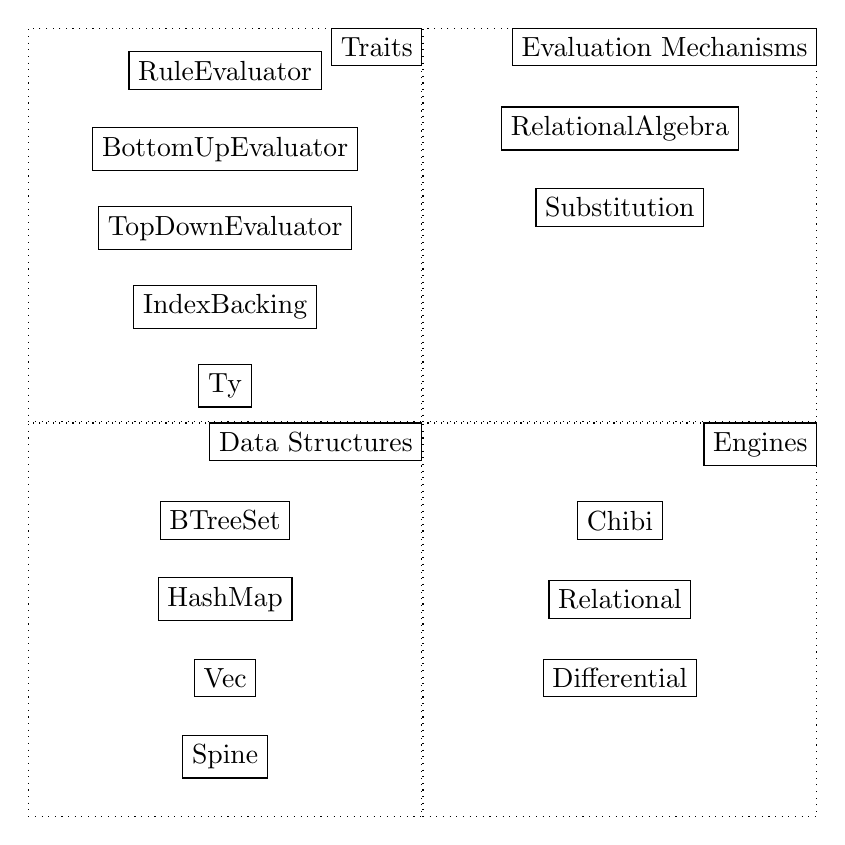
\begin{tikzpicture}
		\begin{scope}
			\node (traits) at (0, 0) [draw, dotted, rectangle, minimum width=5cm, minimum height=5cm] {};
			\node (traits_title) at (traits.north east) [draw, anchor = north east] {Traits};

			\node (ev_mec) at (traits.east) [draw, dotted, rectangle, minimum width=5cm, minimum height=5cm, anchor=west] {};
			\node (ev_mec_title) at (ev_mec.north east) [draw, anchor=north east] {Evaluation Mechanisms};

			\node (ds) at (traits.south) [draw, dotted, rectangle, minimum width=5cm, minimum height=5cm, anchor=north] {};
			\node (ds_title) at (ds.north east) [draw, anchor=north east] {Data Structures};

			\node (engines) at (ds.east) [draw, dotted, rectangle, minimum width=5cm, minimum height=5cm, anchor=west] {};
			\node (engines_title) at (engines.north east) [draw, anchor=north east] {Engines};
		\end{scope}

		% Traits
		\begin{scope}
			\node (insta) [draw, below = 3mm of traits.north] {RuleEvaluator};
			\node (bupe) [draw, below of = insta] {BottomUpEvaluator};
			\node (tode) at (traits) [draw, below of = bupe] {TopDownEvaluator};
			\node (idx) at (traits) [draw, below of = tode] {IndexBacking};
			\node (ty) at (traits.south) [draw, below of = idx] {Ty};
		\end{scope}

		% Data Structures

		\begin{scope}
			\node (btset) [draw, below = 10mm of ds.north] {BTreeSet};
			\node (hashm) at (ds) [draw, below of = btset] {HashMap};
			\node (vecto) at (ds) [draw, below of = hashm] {Vec};
			\node (spine) at (ds) [draw, below of = vecto] {Spine};
		\end{scope}

		% Evaluation Mechanisms

		\begin{scope}
			\node (relal) [draw, below = 10mm of ev_mec.north] {RelationalAlgebra};
			\node (subst) at (ds) [draw, below of = relal] {Substitution};
		\end{scope}

		% Engines

		\begin{scope}
			\node (chibi) [draw, below = 10mm of engines.north] {Chibi};
			\node (relational) at (engines) [draw, below of = chibi] {Relational};
			\node (differential) at (engines) [draw, below of = relational] {Differential};
		\end{scope}

	\end{tikzpicture}
	\caption{Shapiro Components}
	\label{fig:shapiro_comp}
\end{figure}
On figure \ref{fig:shapiro_comp} we can see the most relevant modules. The northwestern quadrant, Traits, refers to Rust Traits, constructs that
define \textit{behavior}, and that can be passed to functions. It is important to take note that Rust favors \textit{composition} over inheritance, unlike Java.
Nevertheless, all other quadrants are built upon these traits, and are therefore generic over any type that implements them.

A \verb|Rule Evaluator| represents $\textbf{T}_p$, requiring only that types implement a function \verb|evaluate|, that accepts an instance,
and produces another instance. The evaluation mechanisms \verb|Relational Algebra| and \verb|Substitution| both implement this trait,
evaluating datalog rules by either using the aforegiven translation algorithm, or using Infer. We also provide naive parallel evaluation of rules,
in which each rule, in both mechanisms, are sent to be executed in a threadpool. We leverage the highly efficient, and easy to use, requiring
only one additional line of code, rayon\cite{rayon} library. This should suffice as a transparent baseline from which other parallelization
strategies could be compared to.

The concept of fixpoint evaluation is a Struct, that consists of the ground fact database, $EDB$, a \verb|Rule Evaluator|, and an array of
instances. It is assumed that the datalog program is in the instance itself. Semi-naive evaluation is a method of fixpoint evaluation that takes
no arguments, and instead uses two additional instances, one to keep the current delta, and the previous one. This is succintly implemented in rust
in the same manner as this description.

\verb|BottomUpEvaluator| and \verb|TopDownEvaluator| both respectively denote the two kinds of evaluation, respectively, the explicit
materialization of the program, and the answering to a query with respect to a program. The former requires the implementation of a function that takes
in only a program as an argument, and the latter, a program and a goal.

The three engines, \verb|Chibi|, \verb|Relational| and \verb|Differential| all implement only \verb|BottomUpEvaluator|. In order to be able to
evaluate a program, it is required to have access to an instance. An instance is defined in code as it is in literature, a set of relations. Taking
inspiration from the highly successful open-source project DataScript\cite{datascript}, we implement relations as hashmaps, with generic hashing
functions. The point of using a hashmap is that it allows for one to easily disregard duplicates altogether, further simplifying the implementation.

Indexes on the other hand, are a vital optimization aspect. A considerable amount of recent datalog research has dealt with speeding up relational joins
with respect to datalog, such as in attempting to specialize data structures to it\cite{souffle_btree}, and rminimizing the number of necessary
joins to evaluate a $SPJ$ expression\cite{primitive_search}. Thus, a trait \verb|IndexBacking| is defined, whose requirements are two methods, one
that takes in a row for insertion, and another that requires a join implementation.

We implement the \verb|IndexBacking| trait for implementations of all most used data structures for datalog indexes, such as the Rust standard
library BTree\cite{rust_btree} and HashMap, persistent implementations of both them, a regular vector, that naively sorts itself before a
join, and the Spine, an experimental data structure, that empirically shows good performance characteristics in datalog workflows.

\subsection{Differential Dataflow}

The \verb|Differential| engine is an attempt at implementing a substitution-based engine on top of the distribution framework that addresses datalog's
evaluation inefficiencies in a manner that no other currently available framework does, differential dataflow\cite{dd}. Most of the distributed datalog engines are
built on top of either graph-processing or map-reduce frameworks, both kinds of projects that were not specifically made with expressive query answering in mind, but
more with efficiently handling complex non-recursive queries over large amounts of data.

One of the biggest challenges in efficiently evaluating datalog is in the deletion of data. Incremental bottom-up processing of additions is already the
manner in which semi-naive evaluation works, and is relatively efficient. The other direction is significantly more complex. In order to delete a fact,
one has to take into account that it might have influenced the inferrence of other facts, which imply having to look over the whole data, while the opposite
direction does not require that, therefore incurring possibly very large performance differences between both directions.

Similarly to how semi-naive evaluation is the \textit{de facto} method for incremental bottom-up evaluation, the Delete-Rederive\cite{dred} algorithm holds
the same regard with respect to the incremental maintenance of bottom-up evaluation with respect to deletions. There are two stages to it, the first, Deletion,
naively overdeletes all facts that could have been derived from it, but at the same time, keeps track of possible facts that could have had alternative
derivations. The second stage, rederive, restarts the evaluation process.

Differential dataflow directly addresses this issue by evaluating both additions and deletions in the same manner, while at the same time efficiently parallelizing
semi-naive evaluation, however, it is first necessary to digress over Timely Dataflow~\cite{timely}, the underlying networked computation system in which differential
is built upon.

Timely is a high-throughput, low-latency streaming-and-distributed model that extends dataflow. The timely in its name refers to it thoroughly establishing
the semantics of each aspect of communication notification, taking the parallelization blueprint and making its execution transparent to the user. A notification
sent between operators is assigned a timestamp, that needs only to be partially ordered, with no assumptions being made with respect to insertion. The goal is to use
them to correctly reason about the data with respect to the local operator states' of computation completion, in order to cleverly know with certainty when not only
whether should work be done asynchronously or with sharding, but whether there is data yet to be processed or not.

Differential Dataflow, a generalization of incremental processing, is an extension to the Timely Dataflow model. While the shape of the data that flows in the latter is
in the form of \verb|(data, timestamp)|, the former's is \verb|(data, timestamp, multiplicity)|, therefore restricting its bag-of-data semantics to multisets, with
the multiplicity element representing a difference, for instance, $+1$ representing the addition of $1$ datapoint arriving at a specific timestamp, or $-1$, a deletion. The
key difference between both models is that similarly to how timely makes distribution transparent, differential does the same with incremental computation, by providing to the
user the possibility of not only adding to a stream, the only possible action in timely dataflow, but allow it to respond to arbitrary additions and retractions at any timestamp.

Similarly to how timestamps in timely are the key element to the efficient parallelization of iterative dataflows, they can also be used in incremental scenarios in order to
overcome their inherently sequential nature. This is of paramount importance to the performance of datalog evaluation.

Let's assume that there is some dataflow that computes the transitive closure of some graph $d_0$, and one update consisted of four edge differences, labeled as $\delta$, arrives, with
the resulting updated graph being $d_1$. In a regular incremental system, each triple would increment the iteration counter by $1$, and even though the relational operations inside
the dataflow might happen in parallel, $\delta_1$, $\delta_2$, $\delta_3$ and $\delta_4$ will only be evaluated after $\delta_0$ and each of its sequent difference's iteration finishes.

If that dataflow were to be executed with differential dataflow, inside the iteration scope there would be a product timestamp $\langle a, b \rangle$, with $a$ representing the time
in which some initial triple was fed into the computation, and $b$ denoting the iteration count, therefore tracking the transitive chain length, respecting the
following partial order: \[\langle a_i, b_1 \rangle \leq \langle a_j, b_j \rangle \iff a_i \leq a_j \wedge b_i \leq b_j\]

If we take that $\delta_0$, $\delta_3$, $\delta_1$ and $\delta_2$ are differences with the following respective timestamps: $\langle 0, 1 \rangle, \langle 0, 2 \rangle, \langle 1, 1 \rangle, \langle 1, 2 \rangle$ it
is noticiable that $\delta_0$ and $\delta_3$ are comparable, but both of them, and vice-versa, are incomparable with respect to $\delta_1$ and $\delta_2$. This, in turn, means that, as it can
these pairs of differences, despite notifying change on the same iteration operator, could safely be executed in parallel in differential dataflow, but not in a regular
incremental system that uses totally-ordered timestamps.

The most notable difference between iterative and incremental processing is that in the latter computation advances by, ideally, making adjustments proportional to the newly
received data, referred to as difference. Naturally, this could result in massively reduced latency, however, in order to support this in the first place, incremental
systems have to maintain indexes of all updates, be it an addition or a retraction, that could impact the calculation.

The differential dataflow implementation, built on top of timely dataflow's rust one, utilizes a novel method to maintain indexes such that they are not restricted
to each individual operator, and could also be shared between multiple readers. This method utilizes shared arrangements, out of which its core concept, collection
trace, is a structure that represents the state of a collection since the latest frontier, as explained in the timely dataflow section, as an append-only ordered sequence
of batches of updates, with each batch possibly being merged with other batches, that make up an LSM-Tree~\cite{lsm}, therefore benefitting from its compaction mechanism
to ensure that only a logarithmic number of batches exist.

\section{Experiments}

The aim of the experiments is to showcase relative performance, and scalability. Given that all reasoners to be compared share as much code as possible, are written in the same
programming language, and use the same elementary memory model, possibly strong empirical statements can be made with respect to the specificities of their implementation.

\textbf{Setup.} The experiments were run on commodity hardware, a MacbookPro with an M1 Pro processor and 16GB of ram, and in no test did swap memory was reached for.
Rust version 1.65 was used.

\begin{table}[]
	\begin{tabular}{llll}
		Dataset    & Area             & Programs   \\
		linux      & program analysis & CSPA, CSDA \\
		postgresql & program analysis & CSPA, CSDA \\
		httpd      & program analysis & CSPA, CSDA \\
		LUBM       & semantic web     & RhoDFS
	\end{tabular}
	\label{table:datasets}
\end{table}

\textbf{Datasets.} On table \ref{table:datasets} all datasets and program names, or acronyms, are shown. There are two areas of interest. The first is program analysis, a highly active research
field that has propelled significant advancements in datalog reasoners, such as \cite{incA}, an incremental datalog engine extended with lattices and recursive aggregates, and
souffle\cite{souffle}, a priceless source of more than half a dozen papers on the engineering aspects of a reasoner. While the latter's point is to run pre-defined programs over
large datasets, the former is meant for more dynamic scenarios, such as in running and maintaining program analyses.

The semantic web has very unique use-cases for datalog, and are the leading source of research in extending datalog. Seeking ways to introduce tuple-generating dependencies to
programs, with evaluation remaining tractable, has been one of the most active research directions, with highly-influential papers establishing new families of datalog
languages\cite{datalog_plus_minus} and thoroughly exploring their complexity classes alongside further expansions\cite{sticky,warded,monadic}.

These advancements have been somewhat tested in practice, albeit with no full reference implementation having been specified. The most comprehensive, and recent, is closed-source\cite{vadalog}.
The leading datalog engine in general, is also closed-source\cite{rdfox}, and is tailored specifically to the semantic web.

\begin{exmp}{Context-sensitive Points-to Analysis Program}
	\begin{align}
		valueFlow(?x, ?y) \leftarrow assign(?x, ?y)                                                 \\
		valueFlow(?x, ?z) \leftarrow assign(?x, ?y), memoryAlias(?y, ?z)                            \\
		valueFlow(?x, ?z) \leftarrow valueFlow(?x, ?y), valueFlow(?y, ?z)                           \\
		memoryAlias(?x, ?w) \leftarrow dereference(?x, ?y), valueAlias(?y, ?z), dereference(?z, ?w) \\
		valueAlias(?y, ?z) \leftarrow valueFlow(?x, ?y), valueFlow(?x, ?z)                          \\
		valueAlias(?y, ?z) \leftarrow valueFlow(?x, ?y), memoryAlias(?x, ?w), valueFlow(?w, ?z)     \\
		valueFlow(?x, ?x) \leftarrow assign(?x, ?y)                                                 \\
		valueFlow(?x, ?x) \leftarrow assign(?y, ?x)                                                 \\
		memoryAlias(?x, ?x) \leftarrow assign(?y, ?x)                                               \\
		memoryAlias(?x, ?x) \leftarrow assign(?x, ?y)
	\end{align}
	\label{program:cspa}
\end{exmp}

\begin{exmp}{Context-sensitive Dataflow Analysis}
	\begin{align}
		null(?x, ?y) \leftarrow nullEdge(?x, ?y) \\
		null(?x, ?y) \leftarrow null(?x, ?y), arc(?y, ?z)
	\end{align}
	\label{program:csda}
\end{exmp}

\begin{exmp}{RhoDFS inference rules}
	\begin{align}
		A(?y, rdf:type, ?x) \leftarrow T(?a, rdfs:domain, ?x), A(?y, ?a, ?z)                                  \\
		A(?z, rdf:type, ?x) \leftarrow T(?a, rdfs:range, ?x), A(?y, ?a, ?z)                                   \\
		T(?x, rdfs:subPropertyOf, ?z) \leftarrow T(?x, rdfs:subPropertyOf, ?y), T(?y, rdfs:subPropertyOf, ?z) \\
		T(?x, rdfs:subClassOf, ?z) \leftarrow T(?x, rdfs:subClassOf, ?y), T(?y, rdfs:subClassOf, ?z)          \\
		A(?z, rdf:type, ?y) \leftarrow T(?x, rdfs:subClassOf, ?y), A(?z, rdf:type, ?x)                        \\
		A(?x, ?b, ?y) \leftarrow T(?a, rdfs:subPropertyOf, ?b), A(?x, ?a, ?y)
	\end{align}
	\label{program:rhodfs}
\end{exmp}

The first program, \ref{program:cspa}\cite{graspan}, expresses pointer analysis, whose goal is to establish which assignments yield value aliases and memory aliases as a reachability problem. Program \ref{program:csda} directly models checking a program's control-flow graph for null edges as a simple transitive-closure computation. The last program, \ref{program:rhodfs}, is used to materialize the non-trivial inference rules from RDFS\cite{rdfs}, a popular data modelling logic for adding semantics to RDF\cite{rdf} data.

\subsection{COST}

\begin{figure}[ht]
	\centering
	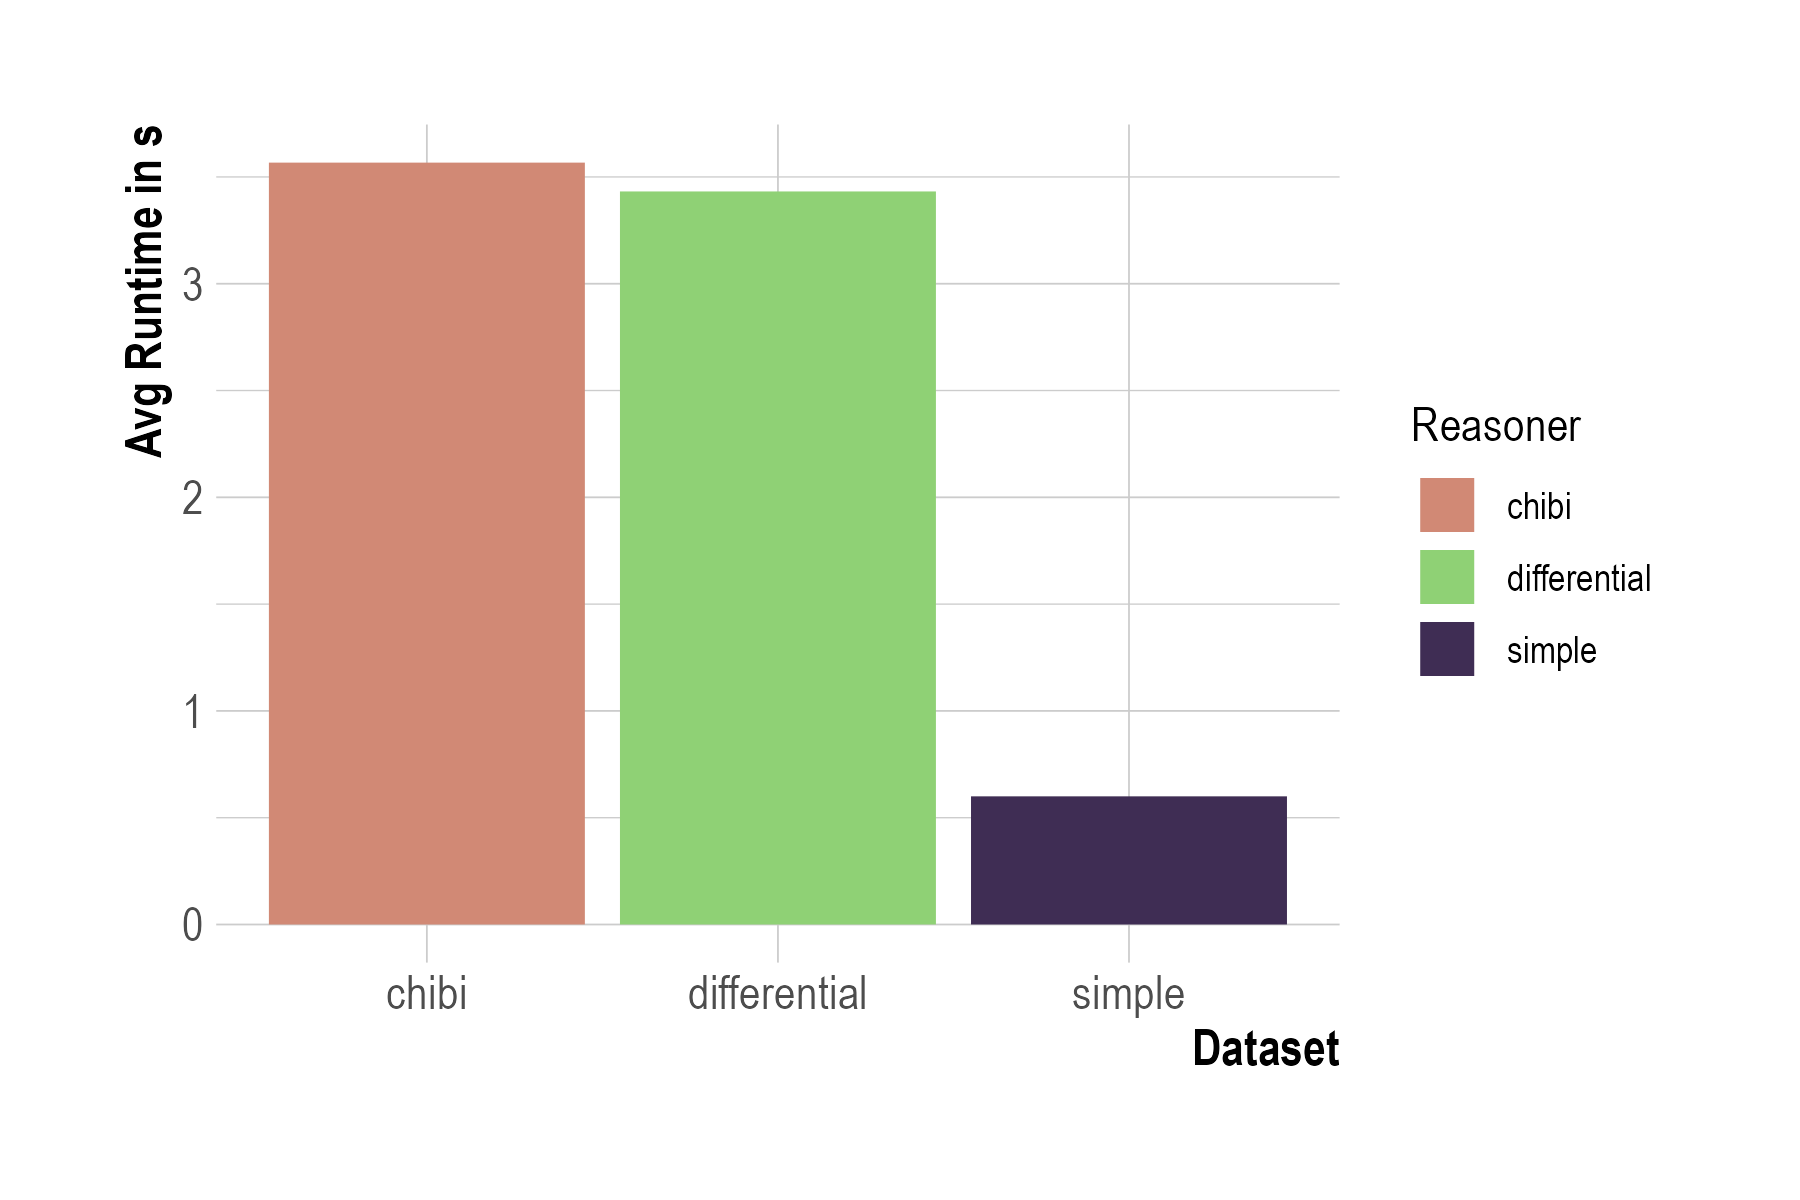
\includegraphics[width=.75\textwidth,height=\textheight,keepaspectratio]{COST}
	\caption{The COST of differential reasoner}
	\label{benchmark:cost}
\end{figure}

Benchmark \cite{benchmark:cost} seeks to answer an important question that is often overlooked, what is the configuration that outperforms a single thread(COST)? this can be convincingly answered in shapiro. As it can be seen, on the LUBM dataset, a synthetic infinitely-scalable ontology, in order to fully materialize all data at once, differential reasoner performs on par with the substitution-based reasoner, showcasing the very little overhead that differential dataflow has, given that it implements the same algorithm as the substitution-based reasoner.

\subsection{Scalability.}

\begin{figure}[ht]
	\centering
	\subfloat[]{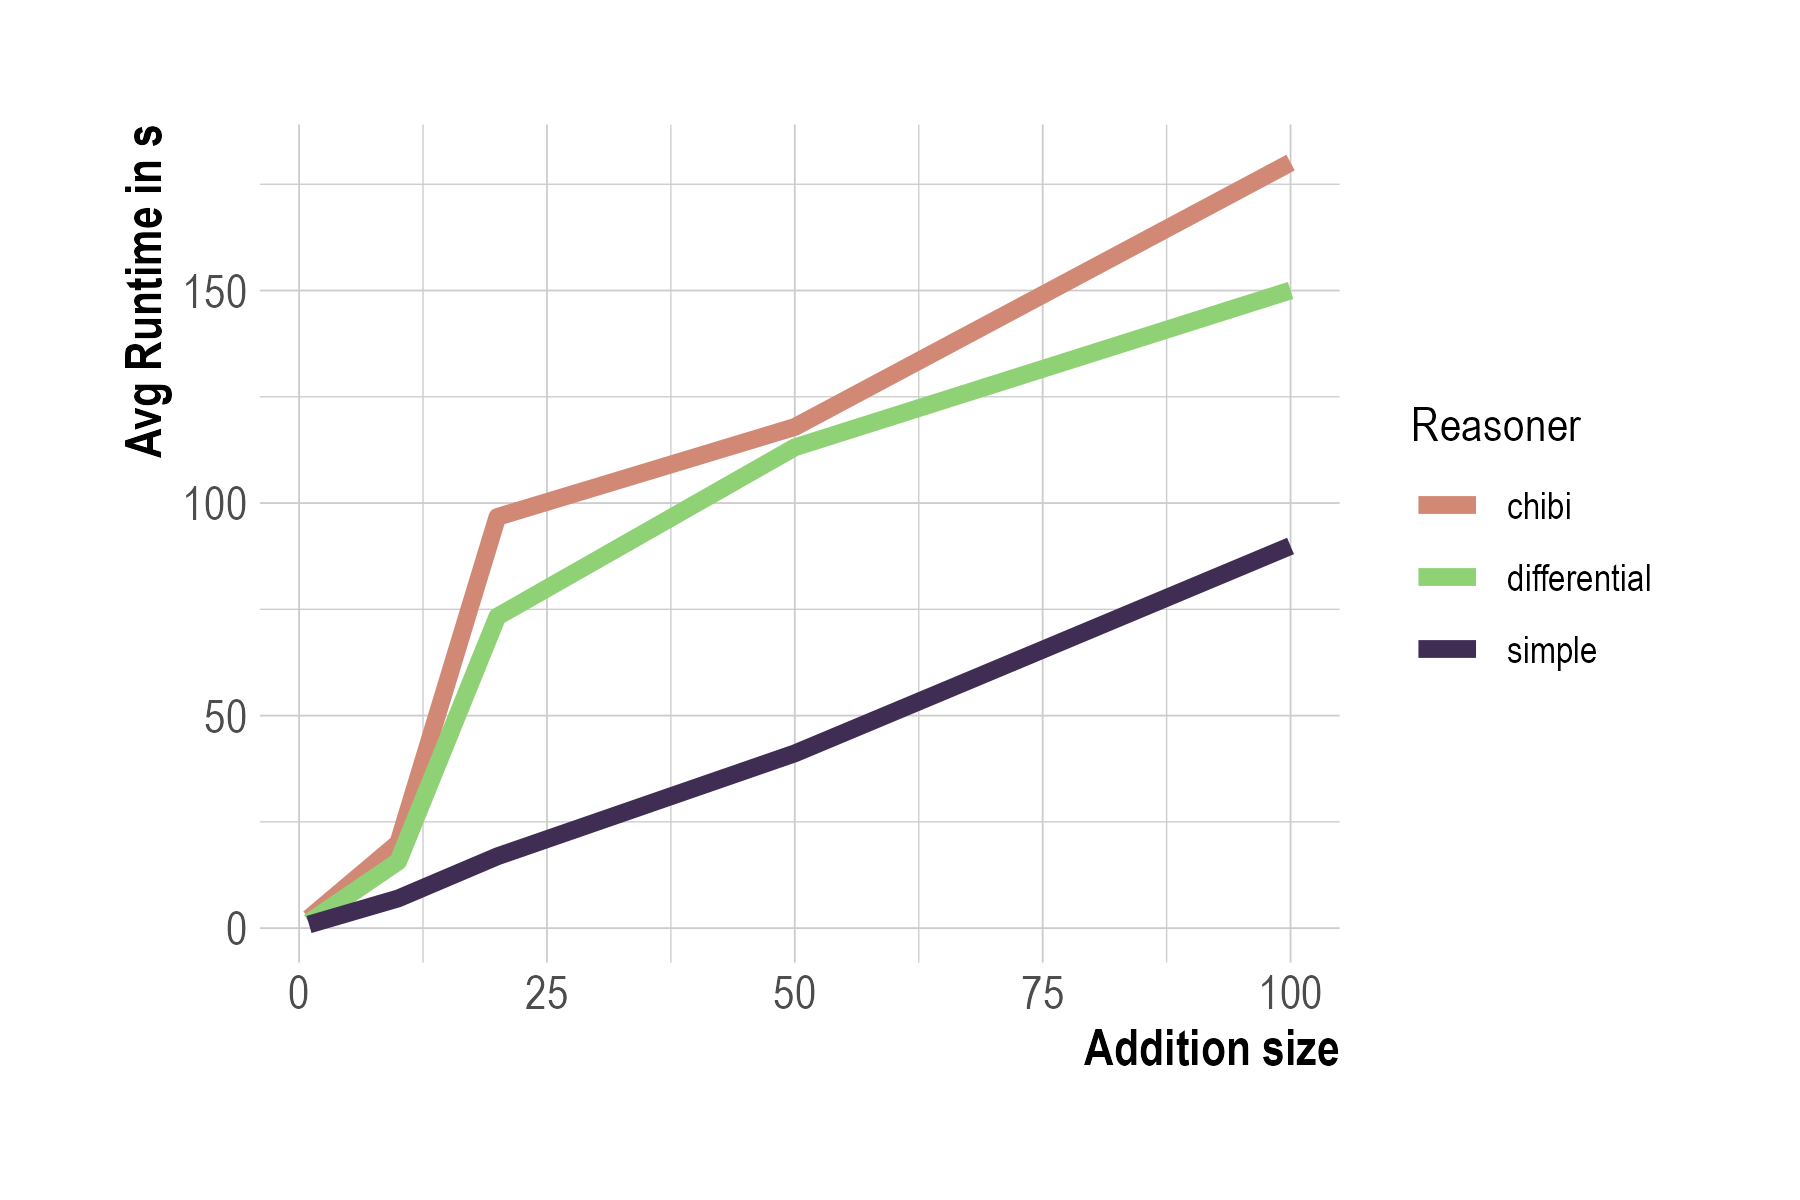
\includegraphics[width=.5\textwidth,height=\textheight,keepaspectratio]{addition}\label{benchmark:scalability_addition}}%
	\subfloat[]{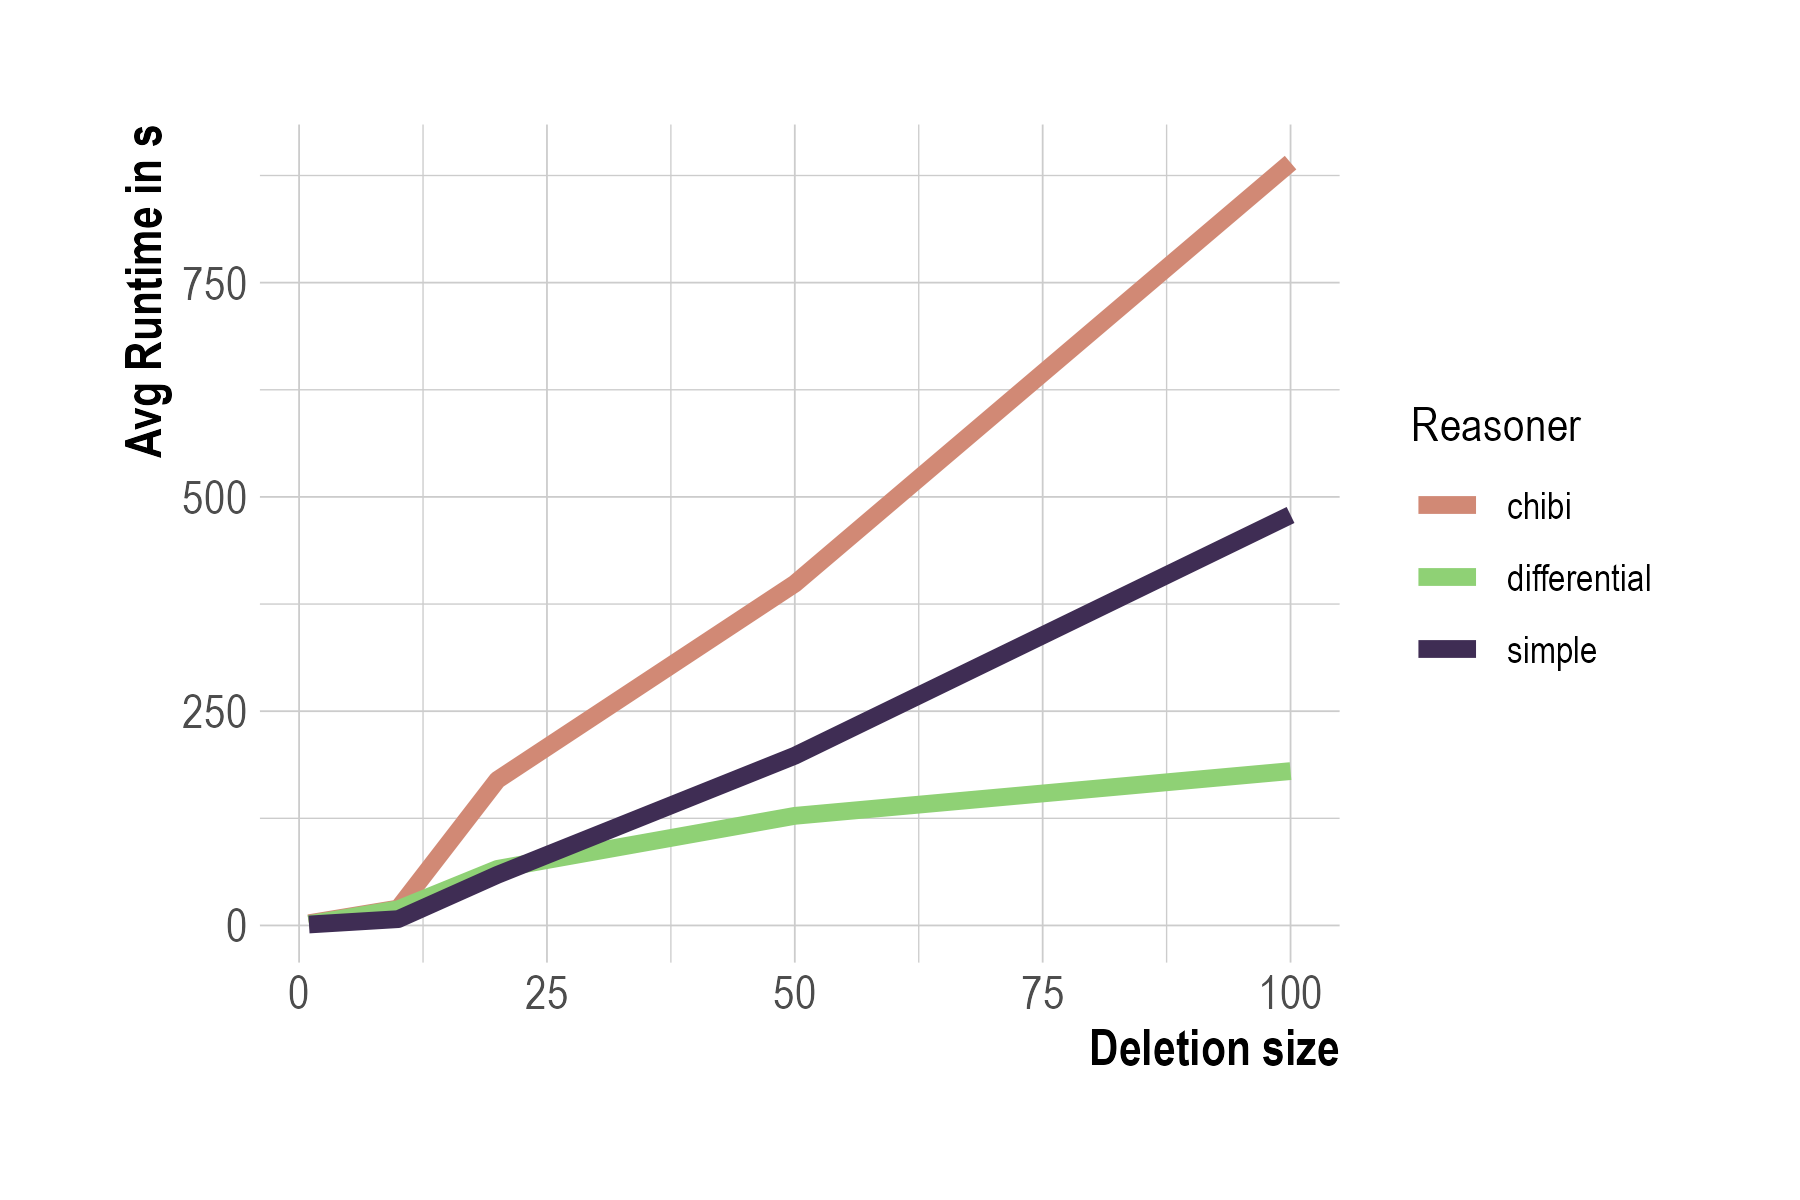
\includegraphics[width=.5\textwidth,height=\textheight,keepaspectratio]{deletion}\label{benchmark:scalability_deletion}}\\
	\caption{Scalability with respect to update size}
	\label{benchmark:scalability}
\end{figure}

Scalability is measured over the LUBM dataset over increasingly larger relative updates. There are two kinds of updates: additions and deletions, both as a percentage of the total data. It is evident from benchmark \cite{benchmark:scalability} that all reasoners scale linearly with respect to the increasing amount of data, however, there is a significant difference with respect to updates. Both non-differential reasoners seem to get polynomially slower with bigger deletion update sizes than differential dataflow.

\subsection{Multiple Datasets.}

\begin{figure}[ht]
	\centering
	\subfloat[]{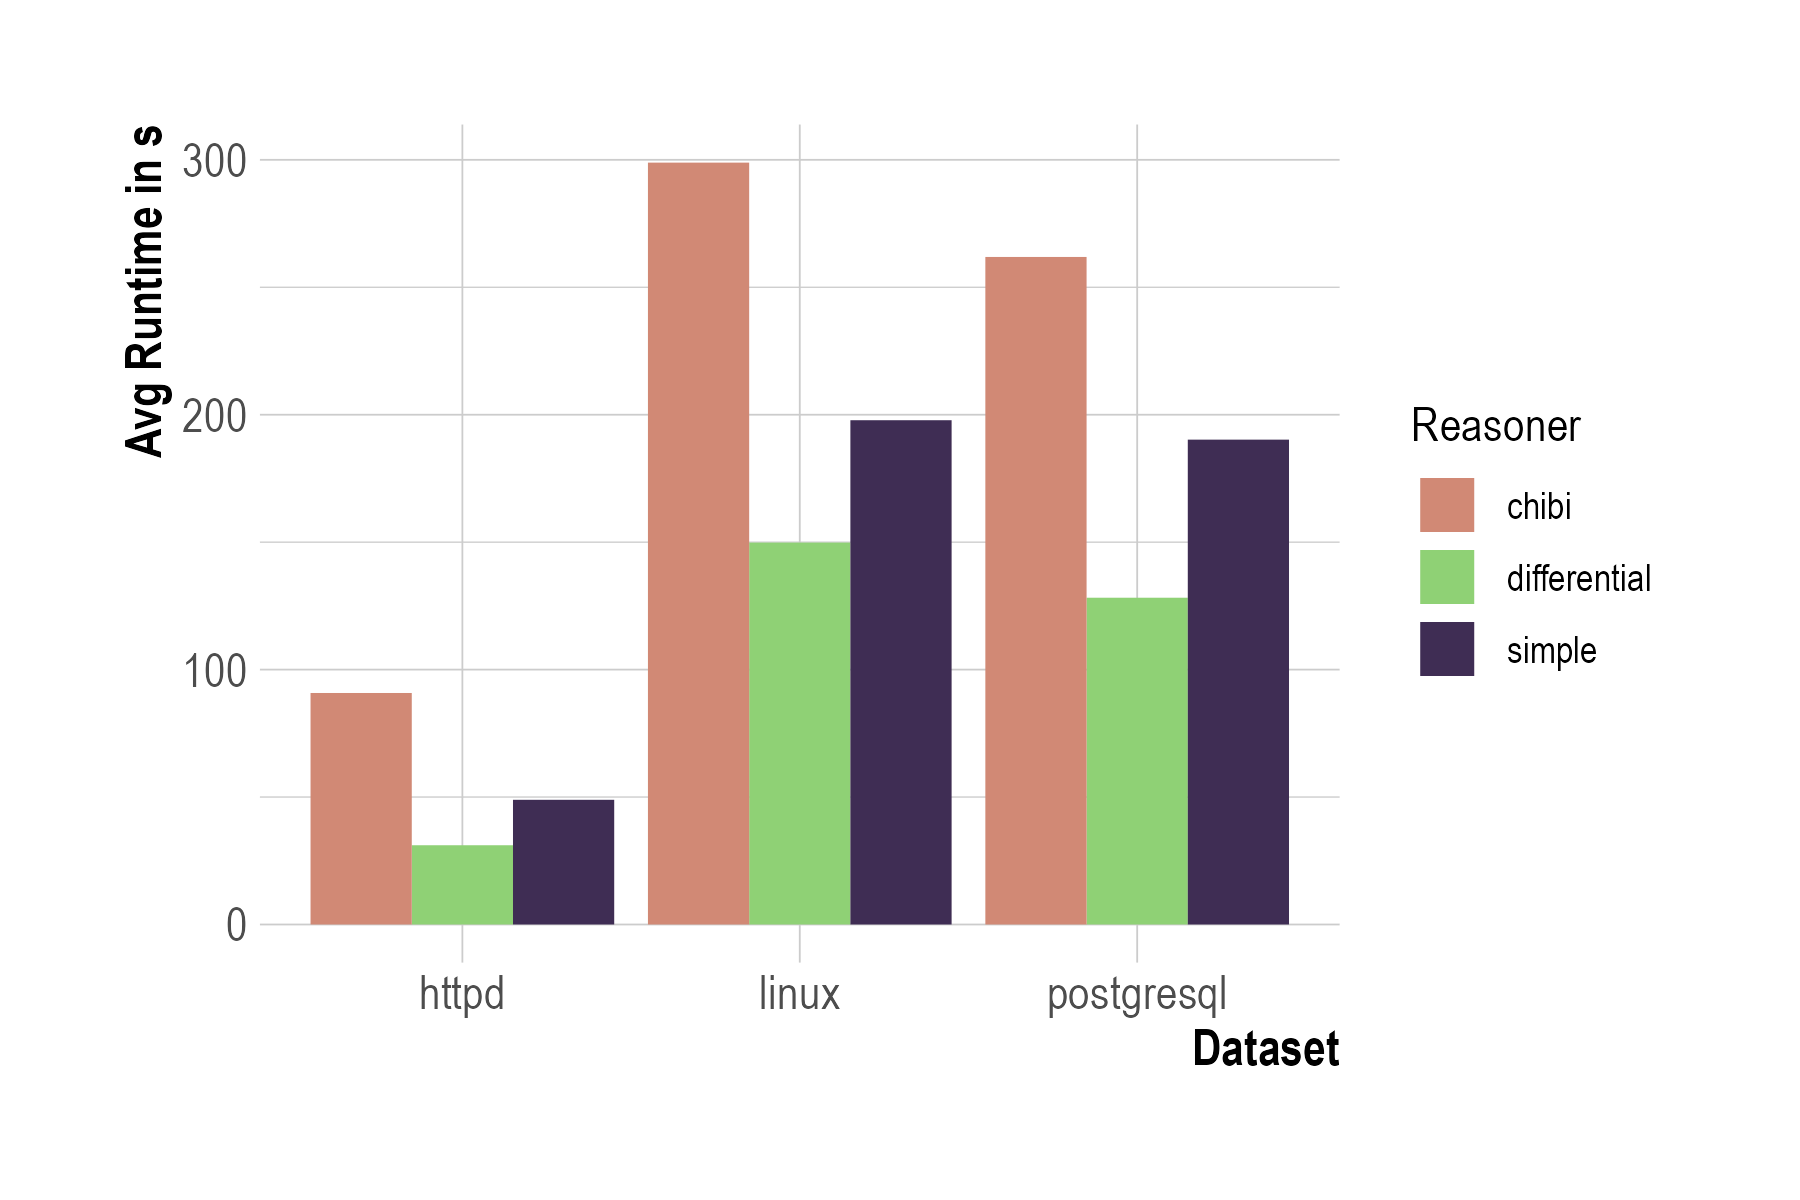
\includegraphics[width=.5\textwidth,height=\textheight,keepaspectratio]{CSDA}\label{benchmark:CSDA}}%
	\subfloat[]{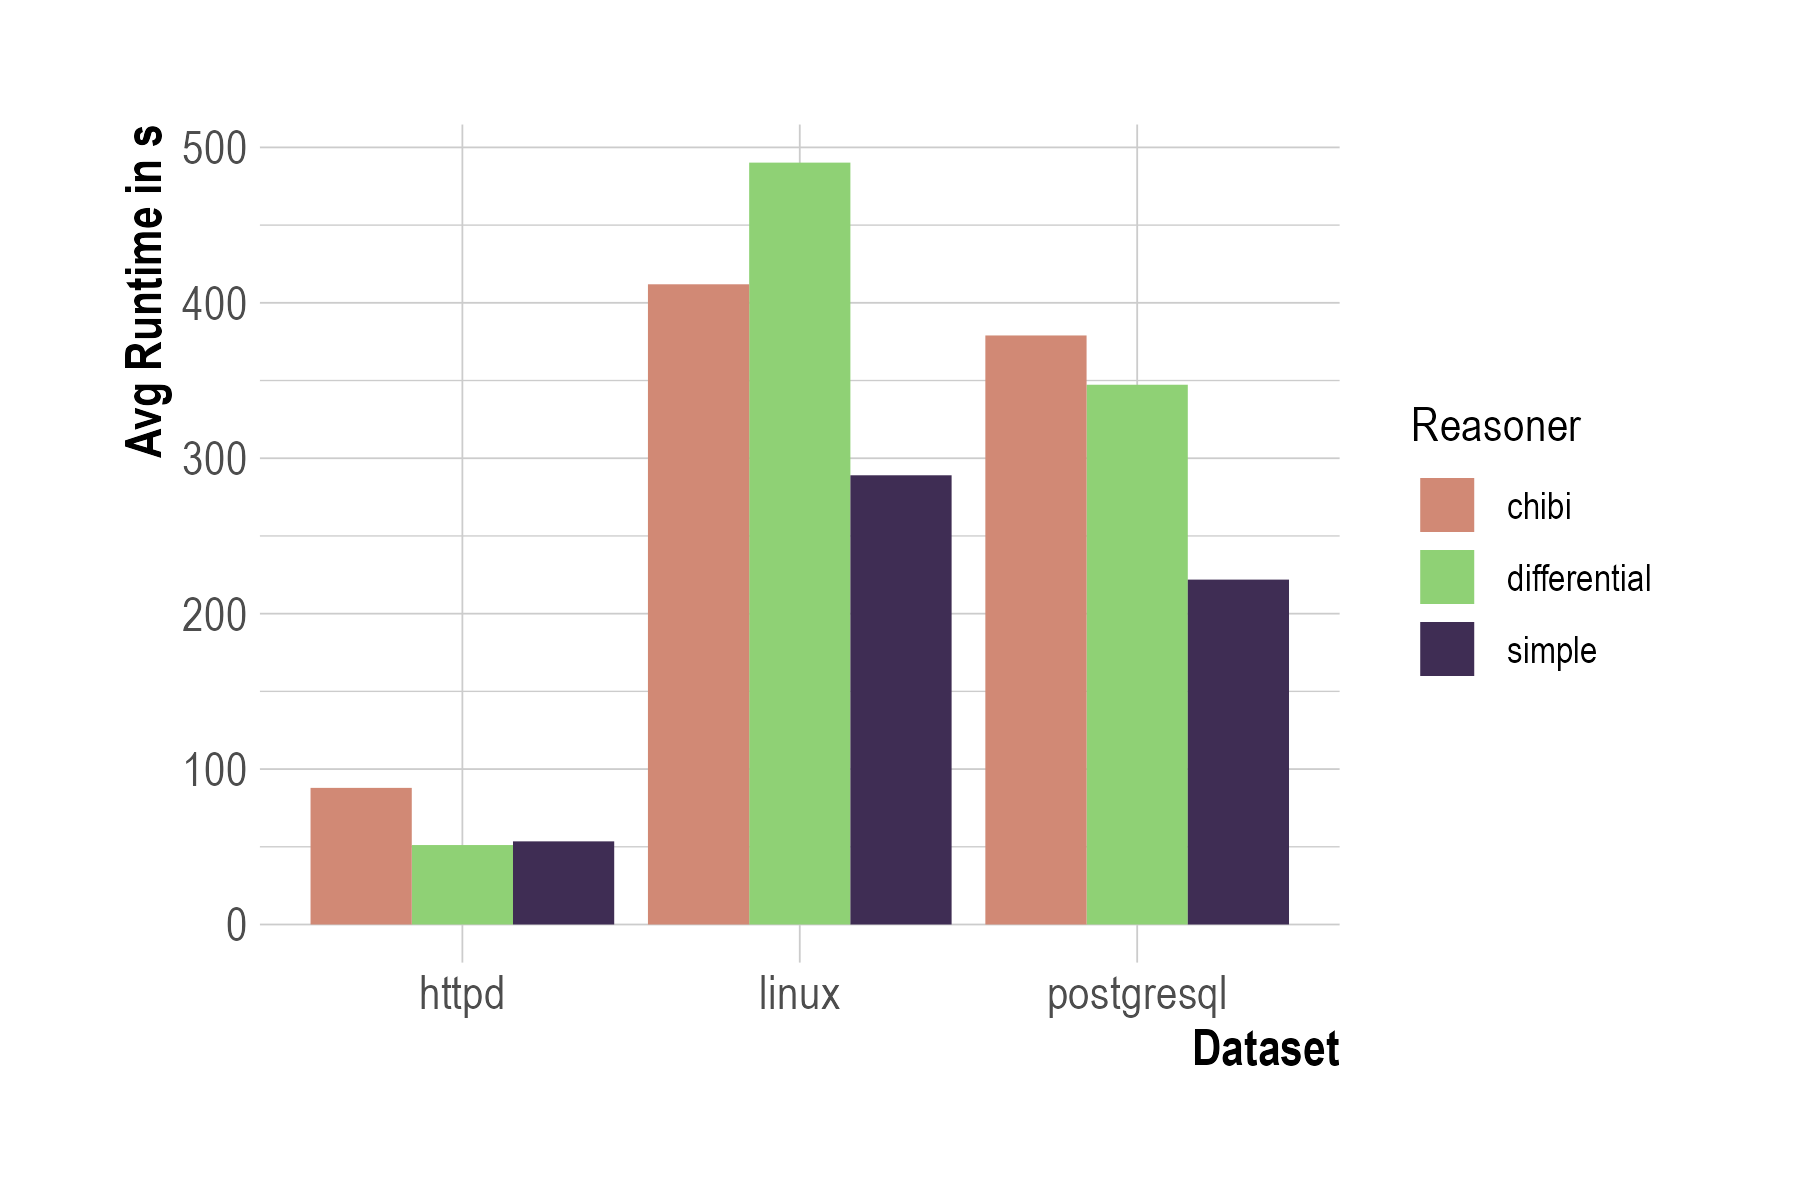
\includegraphics[width=.5\textwidth,height=\textheight,keepaspectratio]{CSPA}\label{benchmark:CSPA}}\\
	\caption{Multiple programs with different datasets}
	\label{benchmark:scalability}
\end{figure}

The last benchmark, pertaining to program analysis, is used to explore the possibly performance differences for completely different datasets, with the same programs. Benchmark \cite{benchmark:csda} is the most surprising, since differential dataflow significantly outperforms the other implementations, while this isn't the case in any other benchmark. The rationale behind that, is that in both non-differential reasoners, iteration implies cloning a non-trivial amount of data, therefore generating a large amount of allocations, while the differential version also makes a large number of allocations, it parallelizes iterations, due to its partially-ordered timestamp, being able to concurrently progress multiple independent transitive chains at once.

\section{Conclusion}

In this paper we introduced Shapiro, a reasoning framework whose core value proposition is in providing modular components to build datalog reasoners. We utilized it to build a reasoner with a promising differential computation framework, differential dataflow, and evaluated it against two other reference implementations. The differential implementation bested its non-differential counterpart, showing very little overhead, however, it did not get close to a relational implementation, the current state-of-the-art approach, nor could it scale as well as the others, nonetheless, it did manage to handle updates in a much more efficient manner, performing exactly as well in additions as in deletions, therefore being much more efficient in practical situations, where no assumption about the kind of update can be made, than both implementations. This yields promising evidence as to the suitability of differential dataflow's computational model to datalog evaluation.

\bibliographystyle{ACM-Reference-Format}
\bibliography{software}

\end{document}
\endinput